\documentclass{article}
\usepackage{tikz}

\begin{document}

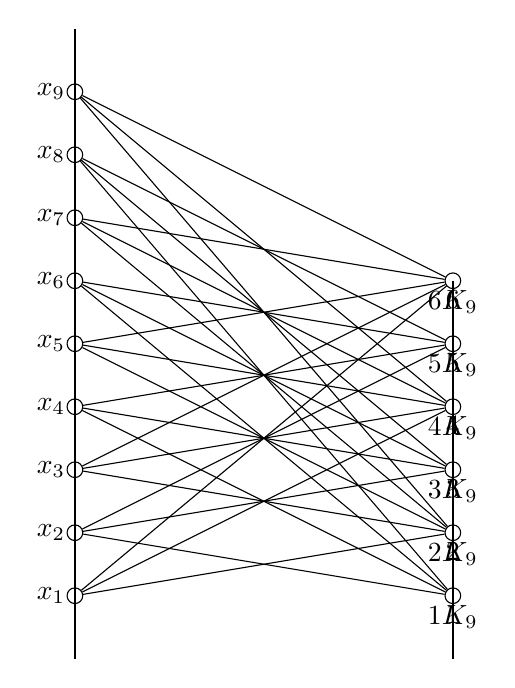
\begin{tikzpicture}[scale=0.8]
    % Define the nodes for the vertical line
    \foreach \y in {1,...,9} {
        \node[circle, draw, fill=white, inner sep=2pt] (v\y) at (-3,\y) {};
    }
    
    % Define the nodes for the horizontal line
    \foreach \x in {1,...,6} {
        \node[circle, draw, fill=white, inner sep=2pt] (h\x) at (3,\x) {};
    }
    
    % Draw the vertical line
    \draw[thick] (-3,0) -- (-3,10);
    
    % Draw the horizontal line
    \draw[thick] (3,0) -- (3,6);
    
    % Draw the edges between the vertical and horizontal lines
    \foreach \y [count=\yi from 1] in {1,...,9} {
        \foreach \x [count=\xi from 1] in {1,...,6} {
            \pgfmathtruncatemacro{\result}{mod(\yi+\xi-1,2)}
            \ifnum\result=0
                \draw (v\yi) -- (h\xi);
            \fi
        }
    }
    
    % Label the vertical nodes
    \foreach \y [count=\yi from 1] in {1,...,9} {
        \node[left] at (-3,\yi) {$x_{\yi}$};
    }
    
    % Label the horizontal nodes
    \foreach \x [count=\xi from 1] in {1,...,6} {
        \node[below] at (3,\x) {$\xi K_9$};
    }
    
    % Label the bottom horizontal nodes
    \foreach \x [count=\xi from 1] in {1,...,6} {
        \node[below] at (3,\x) {$\xi$};
    }
\end{tikzpicture}

\end{document}